\section{Experiments}
\subsection{Experimental Settings}

\paragraph{Benchmarks} We evaluate \ourmethod on 9 benchmarks: MMLU~\citep{hendrycksmeasuring} for general reasoning, GSM8K~\citep{cobbe2021training}, MultiArith~\citep{roy2015solving}, SVAMP~\citep{patel2021nlp}, and AQuA~\citep{ling2017program} for math reasoning, HumanEval~\citep{chen2021evaluating} and DS-1000~\citep{lai2023ds} for code generation, HotpotQA~\citep{yang2018hotpotqa} for web search, and DDXPlus~\citep{fansi2022ddxplus} for medical reasoning.



\begin{table*}[!htbp]
    \centering
    \renewcommand\tabcolsep{5.3pt}
    \renewcommand\arraystretch{1.1}
    \resizebox{\linewidth}{!}{
    \begin{tabular}{lcccccccccc}
    \toprule
    \rowcb
        \textbf{Method}& \textbf{MMLU} & \textbf{GSM8K} & \textbf{MultiArith} & \textbf{SVAMP} & \textbf{AQuA} & \textbf{HumanEval} & \textbf{DS-1000} & \textbf{HotpotQA} & \textbf{DDXPlus} & \textbf{Avg.} \\ \midrule
        Vanilla & 80.47  & 87.15  & 93.40  & 87.25  & 69.27  & 73.28  & 38.40  & 82.35  & 56.40  & 74.22   \\ \hline
        \multicolumn{11}{l}{\textit{\textbf{\small Single-Agent Systems}}}
        \\
        \rowcg
        CoT  & 81.85\red{1.38}  & 87.35\red{0.20}  & 93.60\red{0.20}  & 87.90\red{0.65}  & 72.40\red{3.13}  & 74.05\red{0.77}  & 42.35\red{3.95}  & 81.04\blue{1.31}  & 64.22\red{7.82}  & 76.08   \\ 
        SC & 82.95\red{2.48}  & 87.66\red{0.51}  & 94.40\red{1.00}  & 87.40\red{0.15}  & 71.85\red{2.58}  & 75.82\red{2.54} & 37.66\blue{0.74}  & 82.24\blue{0.11}  & 66.43\red{10.03}  & 76.27   \\ \hline
        \multicolumn{11}{l}{\textit{\textbf{\small Multi-Agent Systems}}}
        \\
        \rowcg
        Chain  & 82.40\red{1.93}  & 87.23\red{0.08}  & 92.88\blue{0.52}  & 87.16\blue{0.09}  & 69.85\red{0.58}  & 73.40\red{0.12}  & 38.25\blue{0.15}  & 80.77\blue{1.58}  & 65.28\red{8.88}  & 75.25   \\ 
        Tree  & 81.55\red{1.08}  & 86.35\blue{0.80} & 92.95\blue{0.45}  & 88.25\red{1.00}  & 71.44\red{2.17}  & 75.33\red{2.05} & 43.50\red{5.10}  & 81.50\blue{0.85} & 69.25\red{12.85}  & 76.68   \\ 
        \rowcg
        Star  & 79.64\blue{0.83}  & 85.25\blue{1.90}  & 93.25\blue{0.15}  & 87.60\red{0.35}  & 68.50\blue{0.77}  & 76.28\red{3.00}  & 41.82\red{3.42}  & 83.52\red{1.17}  & 68.25\red{11.85}  & 76.01   \\ 
        Complete Graph  & 82.75\red{2.28}  & 88.05\red{0.90}  & 94.73\red{1.33}  & 88.20\red{0.95}  & 70.44\red{1.17}  & 84.25\red{10.97}  & 45.05\red{6.65}  & 83.35\red{1.00}  & 70.35\red{13.95}  & 78.57   \\ 
        \rowcg
        Random Graph & 83.20\red{2.73}  & 88.25\red{1.10}  & 94.80\red{1.40}  & 87.10\blue{0.15}  & 70.16\red{0.89}  & 84.14\red{10.86}  & 47.48\red{9.08}  & 84.28\red{1.93}  & 70.44\red{14.04}  & 78.87   \\ 
        AutoGen & 83.25\red{2.78}  & 89.40\red{2.25}  & 95.05\red{1.65}  & 88.15\red{0.90}  & 71.50\red{2.23}  & 83.50\red{10.22}  & 48.55\red{10.15}  & 83.25\red{0.90}  & 71.83\red{15.43}  & 79.39   \\ 
        \rowcg
        LangGraph & 84.10\red{3.63}  & 88.75\red{1.60}  & 95.10\red{1.70}  & 88.03\red{0.78}  & 71.27\red{2.00}  & 84.66\red{11.38}  & 47.95\red{9.55}  & 84.92\red{2.57}  & 72.50\red{16.10}  & 79.70   \\ 
        LLM-Debate & 83.28\red{2.81}  & 89.95\red{2.80}  & 95.45\red{2.05}  & 88.30\red{1.05} & 73.52\red{4.25}  & 85.24\red{11.96}  & 49.26\red{10.86}  & 84.55\red{2.20}  & 71.33\red{14.93}  & 80.10   \\ \hline
        \multicolumn{11}{l}{\textit{\textbf{\small Spatial Evolving Multi-Agent Systems}}}
        \\
        \rowcg
        GPTSwarm & 83.80\red{3.33}  & 90.20\red{3.05}  & 96.28\red{2.88}  & 87.28\red{0.03}  & 75.44\red{6.17}  & 87.14\red{13.86}  & 52.35\red{13.95}  & 85.40\red{3.05}  & 75.57\red{19.17}  & 81.50   \\ 
        G-Designer  & 84.63\red{4.16}  & 93.35\red{6.20}  & 97.60\red{4.20}  & 89.52\red{2.27}  & 76.30\red{7.03}  & 89.40\red{16.12}  & 54.82\red{16.42}  & 87.66\red{5.31}  & 76.42\red{20.02}  & 83.30   \\ 
        \rowcg
        ARG-Designer & \second{85.04}\red{4.57}  & \second{94.40}\red{7.25}  & 97.35\red{3.95}  & 88.95\red{1.70}  & 79.48\red{10.21}  & 88.25\red{14.97}  & \second{55.60}\red{17.20}  & 86.45\red{4.10}  & 76.03\red{19.63}  & 83.51   \\ 
        SafeSieve & 84.65\red{4.18}  & 93.20\red{6.05}  & \second{97.80}
        \red{4.40} & \second{90.10}\red{2.85}  & 80.40\red{11.13}  & 90.15\red{16.87}  & 53.73\red{15.33}  & 87.22\red{4.87}  & \second{77.94}\red{21.54}  & \second{83.91}   \\ \hline
        \multicolumn{11}{l}{\textit{\textbf{\small Temporal Evolving Multi-Agent Systems}}} \\   
        \rowcg
        AFlow & 83.22\red{2.75}  & 89.50\red{2.35}  & 94.28\red{0.88}  & 86.48\blue{0.77} & 78.20\red{8.93}  & 89.25\red{15.97}  & 46.82\red{8.42}  & \second{90.04}\red{7.69}  & 74.25\red{17.85}  & 81.34   \\ 
        SpecReason & 84.20\red{3.73}  & 91.40\red{4.25}  & 95.40\red{2.00}  & 87.62\red{0.37}  & 81.36\red{12.09}  & \second{91.22}\red{17.94}  & 50.08\red{11.68}  & 88.29\red{5.94}  & 76.58\red{20.18}  & 82.91   \\ 
        \rowcg
        STEER & 84.40\red{3.93}  & 93.50\red{6.35}  & 95.82\red{2.42}  & 87.40\red{0.15}  & \second{82.66}\red{13.39}  & 89.02\red{15.74}  & 51.34\red{12.94}  & 89.35\red{7.00}  & 75.20\red{18.80}  & 83.19   \\ \hline
        \multicolumn{11}{l}{\textit{\textbf{\small Spatio-Temporal Evolving Multi-Agent Systems}}} \\   
        \rowcr
        \ourmethod (Ours) & \first{89.85}\red{9.38}  & \first{97.60}\red{10.45}  & \first{99.05}\red{5.65}  & \first{94.72}\red{7.47}  & \first{86.56}\red{17.29}  & \first{94.36}\red{21.08}  & \first{58.65}\red{20.25}  & \first{92.52}\red{10.17}  & \first{82.50}\red{26.10}  & \first{88.42}  \\ \bottomrule
    \end{tabular}}
    \caption{Performance comparison with four types baselines, including Single-Agent Systems, Multi-Agent Systems, Spatial Evolving Multi-Agent Systems, and Temporal Evolving Multi-Agent Systems. All baselines and \ourmethod are driven by self-deployed \llmname{gpt-oss-120b}. \first{Red}: the best, \second{Blue}: the runner-up.}
    \label{tab: main results}
\end{table*}

\paragraph{Baselines} We compare \ourmethod with static approaches like COT~\citep{wei2022chain}, Self-Consistence~\citep{wangself}, Chain, Tree, Star, Complete Graph, Random Graph, AutoGen~\citep{wu2024autogen}, LangGraph~\citep{langgraph}, LLM-Debate~\citep{du2023improving}, Spatial Evolving approaches like GPTSwarm~\citep{zhuge2024gptswarm}, G-Designer~\citep{GDesigner}, ARG-Designer~\citep{li2025assemble}, and SafeSieve~\citep{zhang2025safesieve}, Temporal Evolving approaches like AFlow~\citep{zhangaflow}, SpecReason~\citep{damani2024learning} and STEER~\citep{lee2025confidence}.  

\paragraph{Implementation Details} We run \ourmethod and all baselines with the self-deployed \llmname{gpt‑oss‑120b}. For Temporal Evolving MAS, we access close-source models like \llmname{Qwen3-Max} and \llmname{DeepSeek-V3} through API calls to support model routing. To synthesize dialogue history and generate the final solution, we implement a summarizer agent, maintaining $T=3$ across all baseline comparisons. For the Node Encoder and textual embedding, we adopt \llmname{all-MiniLM-L6-v2} with an embedding dimension of $D=384$. For all datasets, we use 40--80 queries for model training.

\subsection{Main Results}
Results in Table~\ref{tab: main results} demonstrate that \ourmethod achieves consistent state-of-the-art performance across nine benchmarks, with average accuracy improvements from \textit{5.65\%} to \textit{26.10\%}. Compared with Temporal or Spatial Evolving Multi-Agent Systems, \ourmethod possesses more stable performance improvement when faced with heterogeneous tasks, from simple tasks on MultiArith ($5.65 \%\uparrow$) and SVAMP ($7.47\%
\uparrow$) to hard tasks on DS-1000 ($20.25\%\uparrow$) and DDXPlus ($26.10\%\uparrow$). The larger improvements on harder tasks demonstrate the effectiveness of Spatio-Temporal Scheduling.

\subsection{Model Analysis}


\begin{figure}[!htbp]
    \centering

\includegraphics[width=1\linewidth]{Figures/efficiency.pdf}
    \caption{Visualization of performance metrics and token consumption of different multi-agent topologies across MMLU, HumanEval, GSM8K, SVAMP.}
\label{fig: efficiency}
\vspace{-2mm}
\end{figure}
\paragraph{Efficiency Analysis} We analyze the efficiency of \ourmethod in Figure~\ref{fig: efficiency}. When adopting the same number of agents in MAS, \ourmethod outperforms all baselines a lot with less token consumption, showing the capability to fully schedule and utilize the computing resources and specific functions in appropriate moments. Compared with previous advanced baseline ARG-Designer and SafeSieve, \ourmethod only needs nearly $50\%$ of token consumption on MMLU and HumanEval, but with higher accuracy (about $5\% \uparrow$).  We also consider the scalability in Table~\ref{tab: cross comparison}. Results show that the complexities of baselines like GPTSwarm and G-Designer grow linearly as the number of agents increases, while \ourmethod has a lower complexity growth rate, since spatio-temporal scheduling can effectively avoid unnecessary communication during execution.

\paragraph{Robustness Analysis} We validate \ourmethod's robustness in Figure~\ref{fig: stability}. To demonstrate whether the state-aware scheduling is useful, we first conduct experiments on all 9 benchmarks and report the average results of accuracy and stability $e^{\mathcal{R}_{\text{sta}}}$. For approaches, we select G-Designer, ARG-Designer, SafeSieve and \ourmethod since they can be trained using the reward $\mathcal{R}_{\text{sta}}$. 

\begin{figure}[!htbp]
    \centering
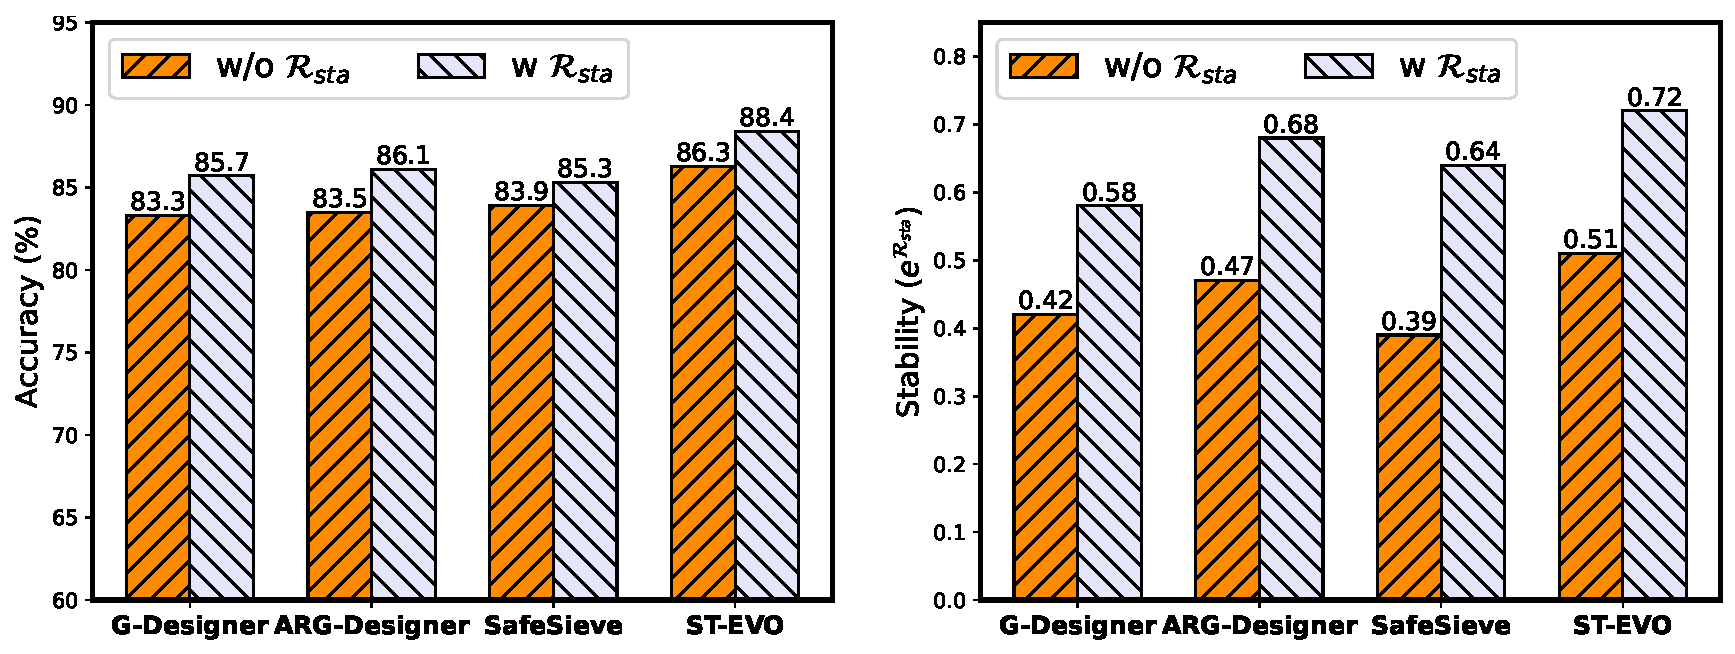
\includegraphics[width=1\linewidth]{Figures/stability.pdf}
    \caption{We utilize the accuracy (\%) and $e^{\mathcal{R}_{\text{sta}}}\in [0,1]$ to visualize the stability of \ourmethod. Higher values indicate better stabilities.}
\label{fig: stability}
\vspace{-2mm}
\end{figure}   
Observations show that all approaches can be improved on both the accuracy and stability using the reward $\mathcal{R}_{\text{sta}}$. This demonstrates that $\mathcal{R}_{\text{sta}}$ can effectively reflect the uncertainty of the MAS, and aligning this preference in Scheduler can lead to generalization on unseen downstream queries. Note that \ourmethod has the most improvement, with about $40\%$ stability improvement. We then conduct experiments to validate whether \ourmethod can fight against external disturbances. Following the experimental settings of prompt injection attack in G-Designer~\citep{GDesigner}, we compare \ourmethod with other baselines in Figure~\ref{fig: robustness}.

\begin{figure}[!htbp]
    \centering
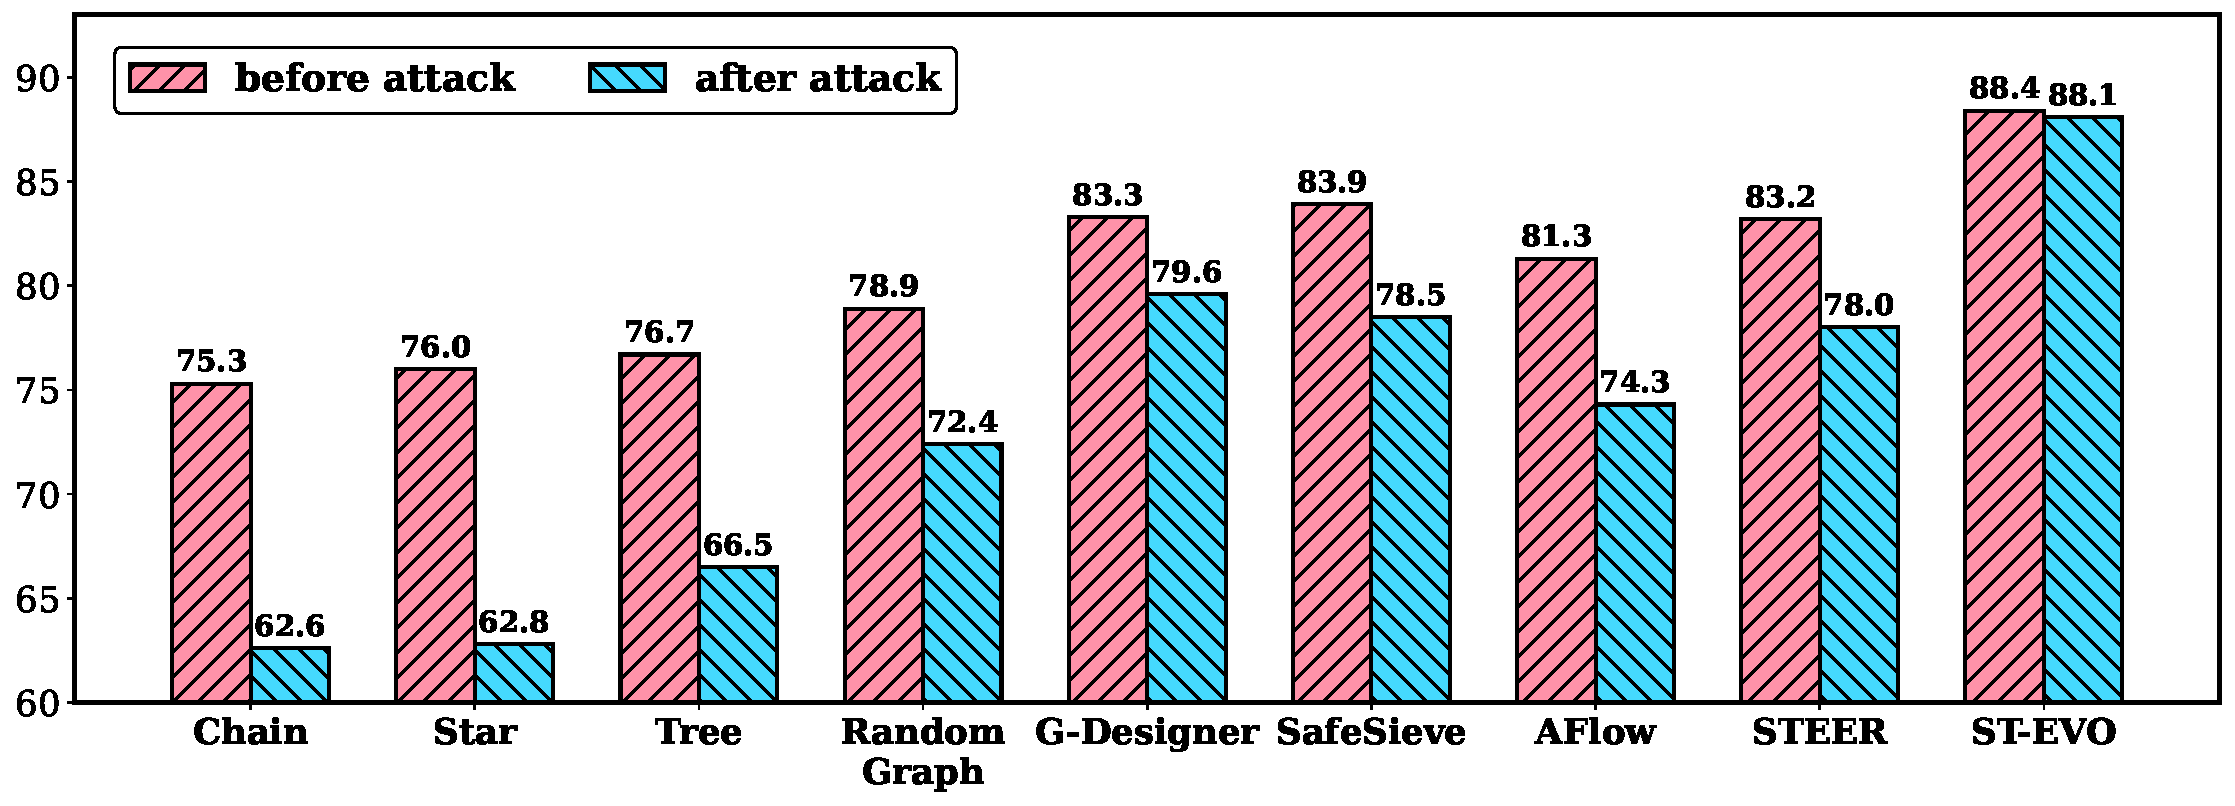
\includegraphics[width=1\linewidth]{Figures/robustness.pdf}
    \caption{We compare the accuracy (\%) of multiple multi-agent systems before and after prompt attacks on all benchmarks, and report the average results.}
\label{fig: robustness}
\vspace{-2mm}
\end{figure}
Results show that static multi-agent systems like Chain, Star, Tree, and Random Graph, suffer significant performance degradation under partial system attacks, with drops about \textit{6.5\%--12.7\%}. Among self-evolving multi-agents, G-Designer and STEER benefit from task-adaptive topology design, only suffer drops under 5\%. Thanks to such adaptive topology adjustment, \ourmethod gains exceptional robustness against adversarial attacks, and can preserve nearly consistent performance before and after the attacks. This advantage can be attributed to the query-wise and state-aware scheduling mechanism, which adds significant flexibility and robustness to the system.

\paragraph{Ablation Study} We conduct ablation studies on \ourmethod--see Table~\ref{tab: ablation}: (1) w/o Scheduling, which limits the Scheduler to output a communication topology for the entire query, (2) w/o $\mathcal{R}_{\text{sta}}$, which does not consider the system uncertainty, (3) w/o $\mathcal{L}_{\text{reg}}$, which does not rely on the experience, and (4) w/o Node Encoder, which removes the task feature $X^{\text{query}}$ in scheduling, and using adaptive representations to replace the node features.

\begin{table}[!htbp]
\centering
\resizebox{0.95\linewidth}{!}{
\begin{tabular}{l|cccc}
\toprule
Variant & MMLU & HumanEval & SVAMP & GSM8K\\ \midrule 
\ourmethod & 89.9 & 94.4 & 94.7 & 97.6 \\ \midrule
\textit{w/o} Scheduling & 84.7 & 89.6 & 88.6 & 92.5\\
\textit{w/o} $\mathcal{R}_{\text{sta}}$ & 87.3 & 90.2 & 91.5 & 95.8  \\
\textit{w/o} $\mathcal{L}_{\text{reg}}$ & 84.9 & 88.2 & 90.3 & 93.7 \\ 
\textit{w/o} Node Encoder & 82.0 & 84.8 & 87.5 & 94.8\\
\bottomrule
\end{tabular}}
\caption{Ablation study tested on MMLU, HumanEval, SVAMP, and GSM8K benchmarks.}
\label{tab: ablation}
\vspace{-2mm}
\end{table}
We observe that w/o Scheduing and w/o Node Encoder matters a lot, because the lack of them would break the core query-adaptive Spatio-Temporal Scheduling mechanism of \ourmethod. w/o $\mathcal{R}_{\text{sta}}$ and w/o $\mathcal{L}_{\text{reg}}$ may also make the MAS vulnerable to interference, thus degrading the performace.


